\section{Results}

We now consider the motion of an orbiter about Europa which is orbiting Jupiter at the same time. The parameters for this environment have been obtained from JPL SSD database \cite{jplssd} for the parameters pertaining the 2-body motion and Schubert \cite{schubert2004interior} for the radius of Europa and the $J_2$ coefficient. A especial perturbations approach was implemented that numerically integrates equations \ref{eomX}-\ref{eomZ}, details can be found on Annex \ref{annexCode}.

For reference on the non-dimensional units, the period of the orbit of Europa about Jupiter is $3.55$ days, the non-dimensional distance is $19.6 \times 10^3$ km and the radius of the satellite is $1565$ km. In non-dimensional units, its radius is close to $.08$ and an an altitude of $200$km is about $0.01$ units.

\subsection{Stable case results}
As a first validation of the theory, we start by comparing the motion for the stable case. We consider an orbiter around Europa with an eccentricity of 0.1 and an altitude of $400$ km, ($a=0.1$) and an null initial argument of periapsis. This scenario corresponds to $\chi = .2746, \alpha = 3.4080$ used for the phase plane in the stable case. We perform an integration for long enough for the eccentricity to complete one revolution and we compare it with the analytical results in figure \ref{fig:stableEccentricityComparison}.

\begin{figure}[H]
	\centering
	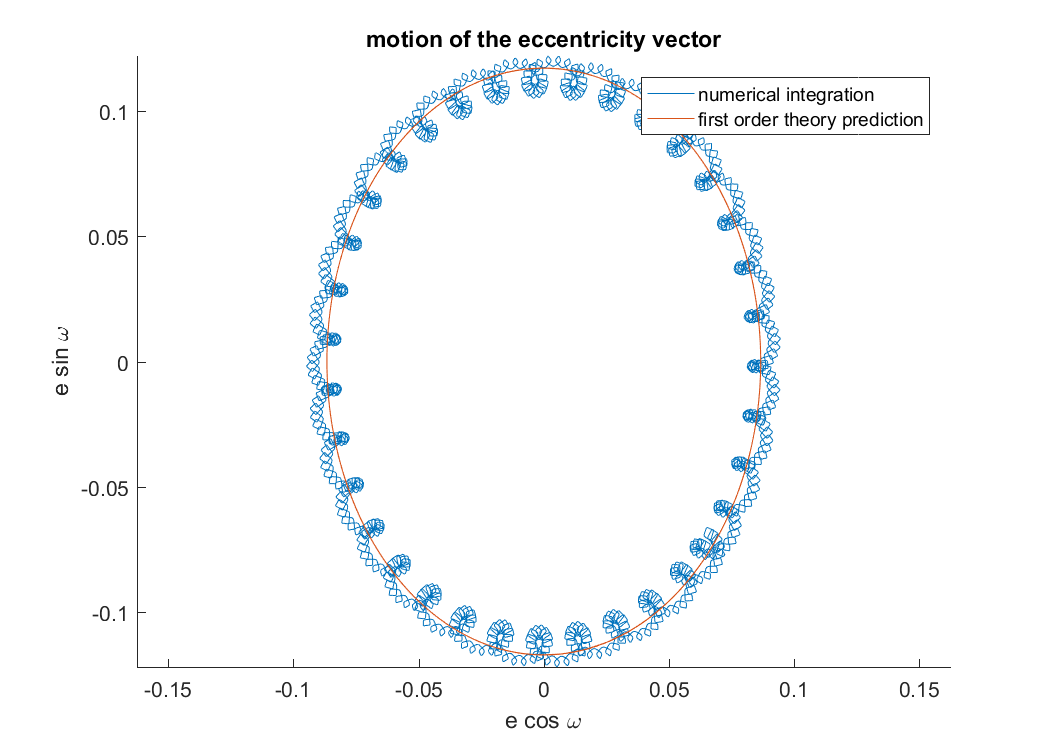
\includegraphics[height=3in]
	{figures/Europe400km01e30i/eccentricityComparison.png}
	\caption{Comparison of the motion of the eccentricity vector for a stable case between first order theory and especial perturbations. The theory predicts accurately the mean motion of the eccentricity.}
	\label{fig:stableEccentricityComparison}
\end{figure}

We observe that the motion resulting from the numerical integrations fits pretty well the predictions of the analytical theory. We must have into account that analytical theory works with the mean eccentricity which will differ from the actual eccentricity due to short term perturbations which have been averaged. We also show in figure \ref{fig:stableEelements} that the semimajor axis and inclination stay constant in mean as predicted by theory.

\begin{figure}[H]
	\centering
	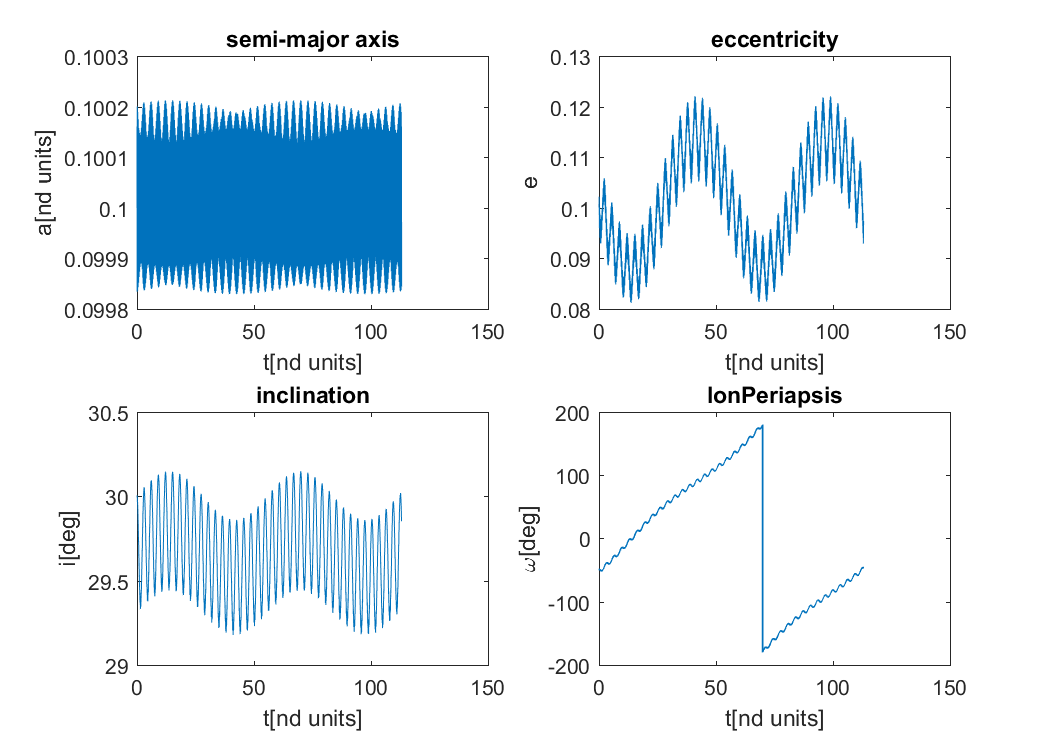
\includegraphics[height=3in]
	{figures/Europe400km01e30i/elements.png}
	\caption{Evolution of the orbital elements: the semi-major axis and inclination remain constant in average as predicted by the theory.}
	\label{fig:stableEelements}
\end{figure}

\subsection{Unstable case results}

This is the case of high inclination orbits which is of greatest interest to the case of a sciencific mission. Since the eccentricity will be unstable for high inclinations, this will lead to decreasing altitudes in the periapsis and eventually to an impact against the satellite. In order to maximize the return of the mission, we would like to maximize the time to impact of the orbiter. The condition for impact is for the periapsis to reach surface radius, assuming the planet is a perfect sphere for this purpose. This condition can be expressed in terms of eccentricity for a given semi-major axis:
\begin{equation}
e_f = 1-\frac{r_{sat}}{a}
\end{equation}

From the analytic theory, we know this will be achieved if we start in a circular orbit or if we start in the attractive manifold. From a mission design perspective, the latter would be more interesting since we would first have to arrive to the circular orbit anyway. Thus, the initial condition can be chosen on the attractive manifold, the injection into the satellite should be made in a way that the elliptic orbit has the right argument of periapsis, this the approach followed in JUICE \cite{esa2011juice}.

This behavior is showcased with an orbiter around Europa with an initial eccentricity of 0.1 and an altitude of $200$ km, ($a=0.09$) which is close to impact and an initial argument of periapsis such that the satellite is on the attractive manifold. This scenario corresponds to $\chi = 0.4650, \alpha = 0.1287$ used for the phase plane in the unstable case. We perform an integration for long enough for the eccentricity to increase and cause an impact the surface. In the case of the averaged analytical theory, if the initial conditions are chosen exactly on the manifold then the trajectory is convergent to the equilibrium, instead a perturbation equal to the observed short term oscillations in the eccentricity is introduced.

The impact condition happens when the eccentricity reaches $0.1178$. The results between match closely, the non dimensional time to impact in the averaged model is $115$ units, and $117$ for the numeric integration, an error below $1\%$ , also the motion of the eccentricity vector matches well the motion of the analytic model as shown in figure \ref{fig:unstableEccentricityComparison}. 

\begin{figure}[H]
	\centering
	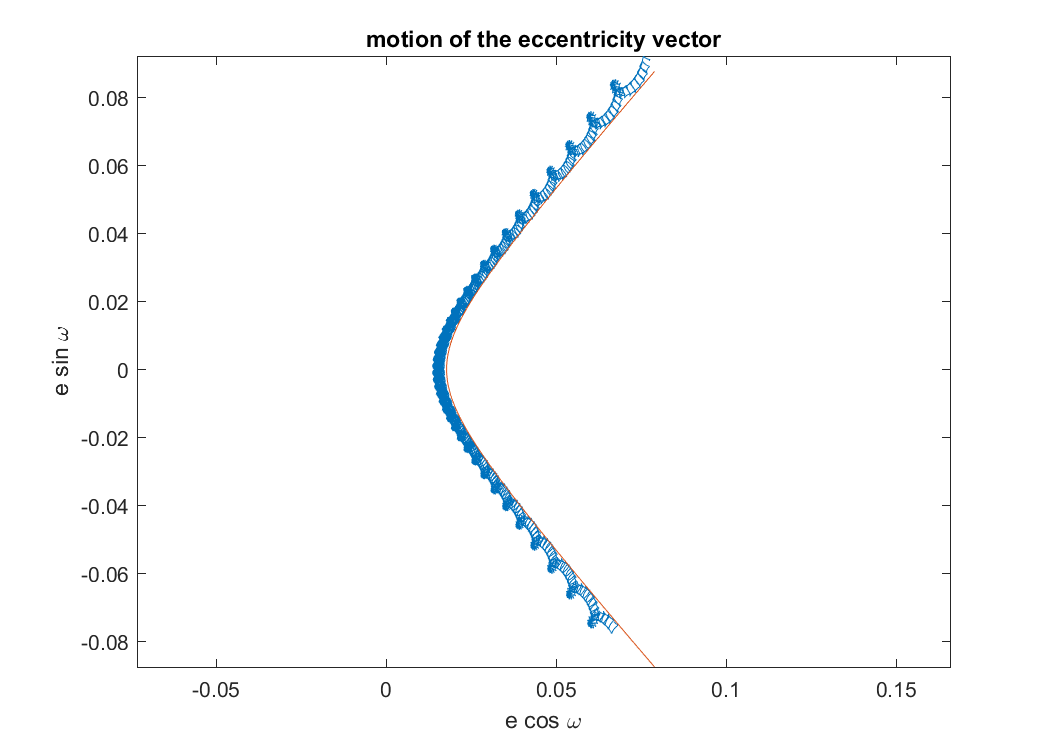
\includegraphics[height=3in]
	{figures/Europa200km01e60i/eccentricityComparison.png}
	\caption{Comparison of the motion of the eccentricity vector for a stable case between first order theory and especial perturbations. Short term perturbations seem to limit the effectiveness of the attractive manifold.}
	\label{fig:unstableEccentricityComparison}
\end{figure}

We also observe that the other elements behave as expected: the semi-major axis and inclination remain constant as shown in figure \ref{fig:elementsUnstable}.

\begin{figure}[H]
	\centering
	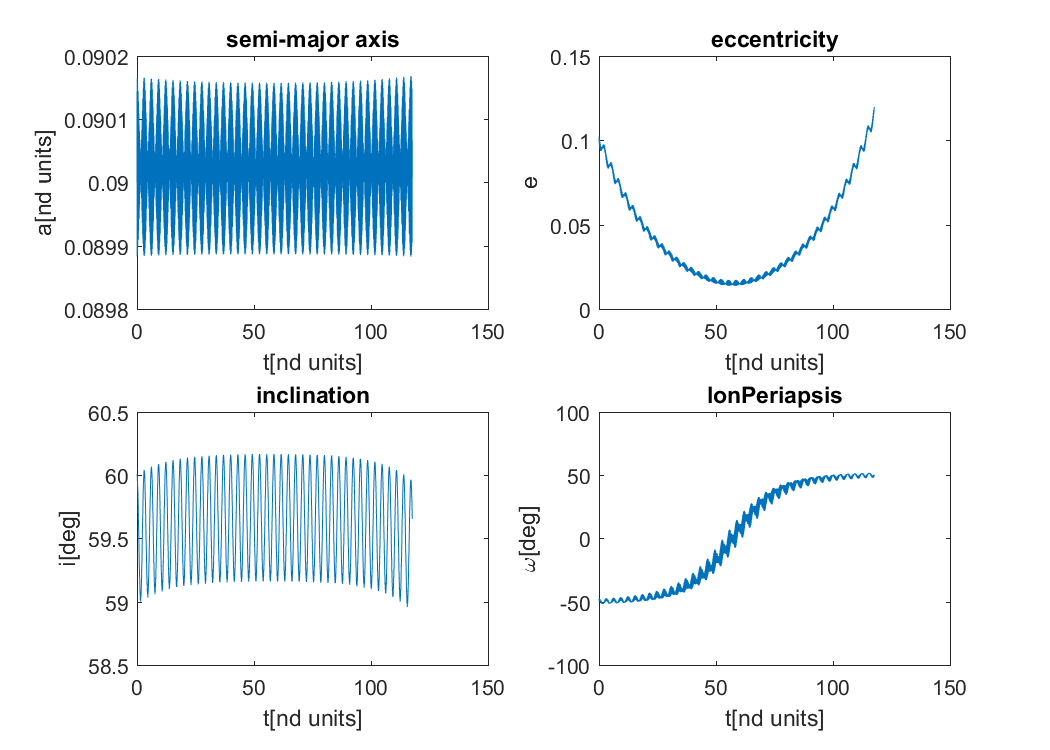
\includegraphics[height=3in]
	{figures/Europa200km01e60i/elements.png}
	\caption{Evolution of the orbital elements: the semi-major axis and inclination remain constant in average as predicted by the theory.}
	\label{fig:elementsUnstable}
\end{figure}

We note initial conditions were chosen to be on the envelope of the short terms oscillations for the analytical model and provide a good fit. This reinforces the idea that the short term perturbations excite the unstable modes and limit the lifetime of the satellite. Another source for this error could be the that the mean argument of the periapsis is not exactly on the attractive manifold due to short term perturbations. For a closer analysis of this effect, it would necessary to find the expressions for the short term perturbations in terms of the anomaly of the orbit and the latitude of the ascending node. This could lead to better choices of the initial conditions that increase the lifetime. The last test will on this.

\subsection{Application to higher altitude orbits: JUICE mission profiles}

As a final test, we change the scenario to that of JUICE orbiting Ganymede. In \cite{esa2011juice} the mission altitude profile for the beginning of the orbit is given. This consists on an elliptical injection into a $200\times10000$ km altitude orbit in the stable manifold that will circularize the orbit, the circular orbit is maintained by means of the AOCS system and finally the orbit evolves into a $200\times 10000$ altitude orbit. In non-dimensional units the semi-major axis of the orbit is $a\approx.167$ and the $200$ km altitude is $ r \approx 0.062$. With these conditions the eccentricity is $e \approx .63$. These clearly violate the assumptions of small eccentricity introduced for the development of the theory.

We obtain the attractive and unstable globalized manifolds by integrating for negative and positive time respectively from a purely circular orbit until the maximum eccentricity is obtained. The mission profile shown in figure \ref{fig:missionProfile}resembles that of ESA to a large extent, if we remove the periodic bits where the AOCS is assumed to be acting, the natural evolution of the orbit is about 90 days.

\begin{figure}[H]
	\centering
	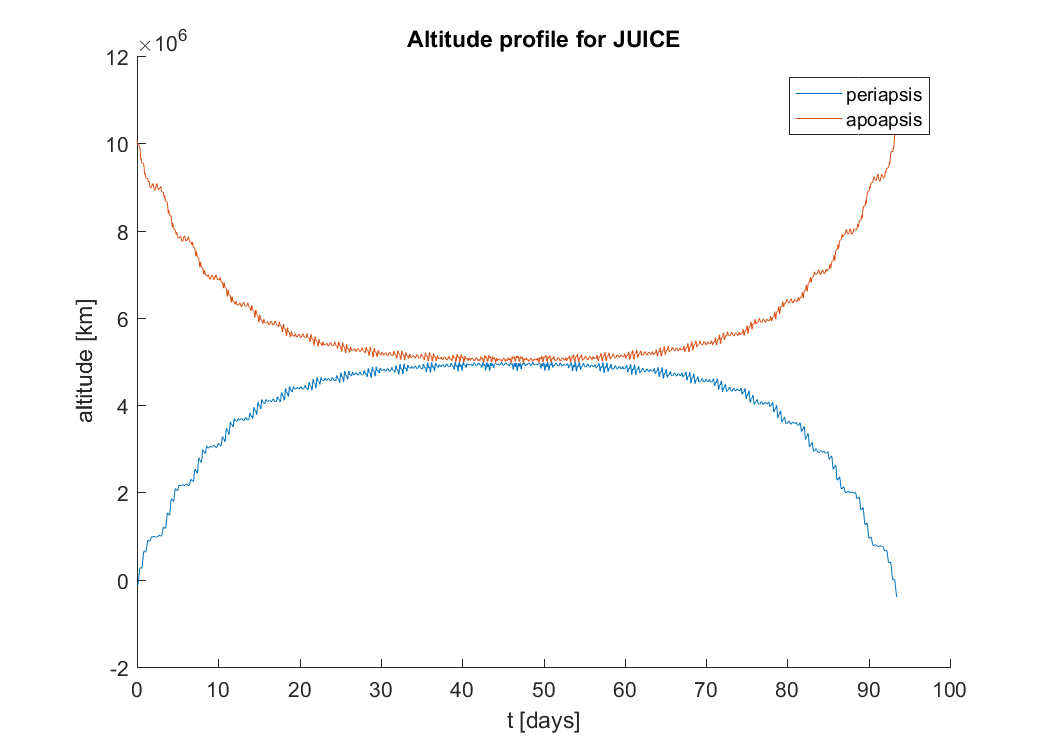
\includegraphics[height=3in]
	{figures/GanymedeESA/missionProfile.png}
	\caption{Altitude profile for JUICE mission from orbit injection to first major maneuver from our model. Reproducing to ESA \cite{esa2011juice}, figure 7-8}
	\label{fig:missionProfile}
\end{figure}

In order assess the accuracy of the theory for greater eccentricities, we compare two things: the differences in the phase plane of the eccentricity and differences in the time evolution of the system. In the phase plane we know that for small eccentricities the argument of periapsis for the manifolds is constant, but as we globalize for greater eccentricities this doesn't have to hold. In figure \ref{fig:eccentricityComparisonGlobal} this is done for one trajectory, we observe that the argument of periapsis for the manifolds starts to drift slowly but being sufficiently close, but the short term perturbation increase with eccentricity, as can be expected from our small eccentricity assumption. 

\begin{figure}[H]
	\centering
	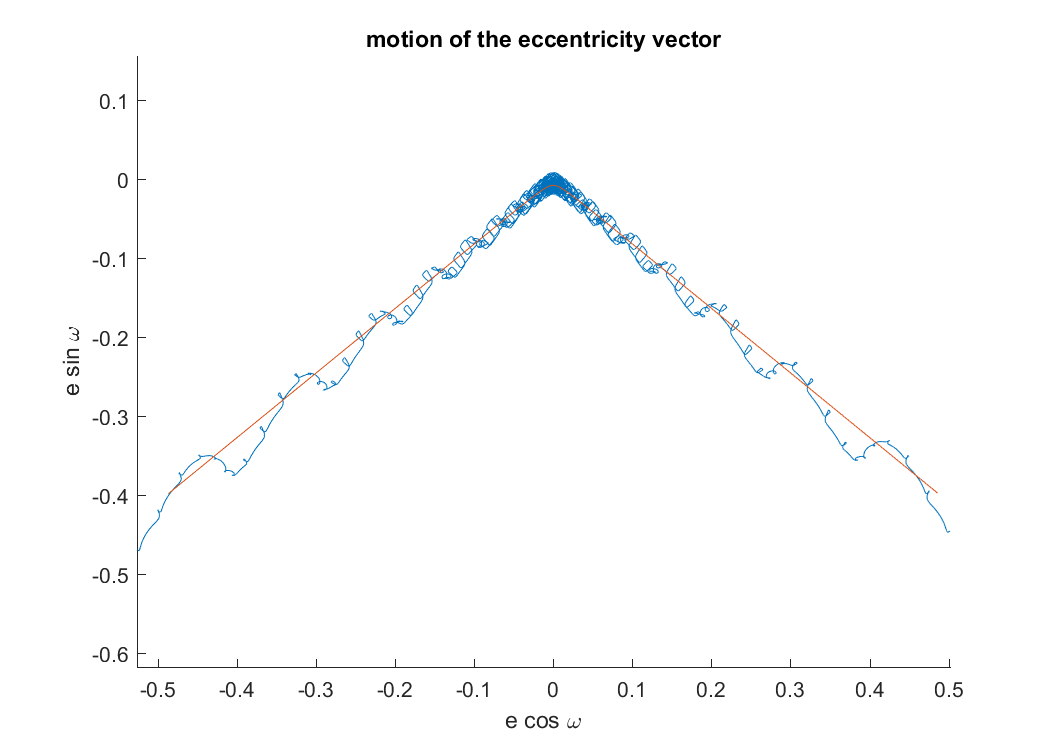
\includegraphics[height=3in]
	{figures/GanymedeESA/eccentricityComparison.png}
	\caption{Phase plane for high eccentricities. The averaged behavior resembles the behavior of the global manifolds but differences begin to show.}
	\label{fig:eccentricityComparisonGlobal}
\end{figure}

Even if a phase portrait is similar, there may be important differences in the rates of convergence and divergence as the manifolds are globalized. To asses this, we compare the time evolution of the altitude profile obtained from the numerical integration with the eccentricity predicted by the first-order theory. We compare the evolution of the profile for the first 40 days of the mission, when it is converging to the circular orbit. Figure \ref{fig:missionProfileTheoretical} shows that the difference is small, meaning that the time evolution doesn't change greatly.

\begin{figure}[H]
	\centering
	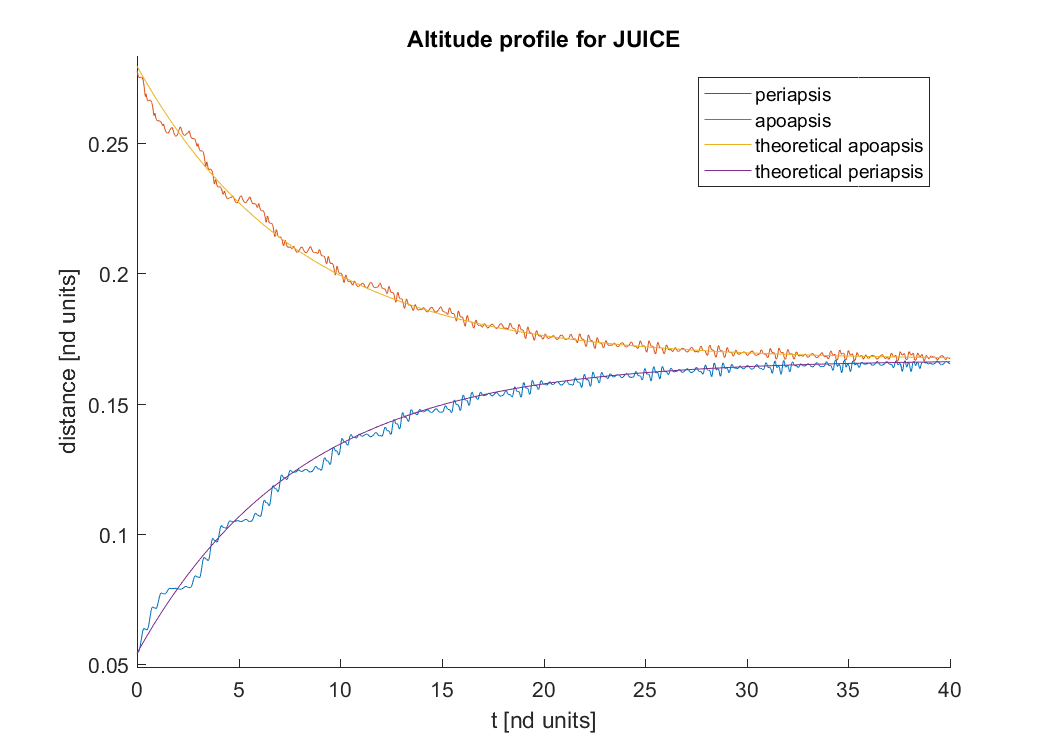
\includegraphics[height=3in]
	{figures/GanymedeESA/missionProfileTheoretical.png}
	\caption{Altitude profile for the mission compared with the prediction from the small eccentricity theory.}
	\label{fig:missionProfileTheoretical}
\end{figure}

Overall, we can state that the insight the developed analytical theory still applies for higher eccentricity orbits. However, the difference in the time to impact between initial conditions chosen a priori and those obtained from globalizing the manifolds has increased significantly. Meaning that especial perturbation methods become increasingly more accurate and necessary for mission design. Figure \ref{fig:JUICEorbit} shows the orbit in a non-rotating frame where the changes in the eccentricity vector can be appreciated.

\begin{figure}[H]
	\centering
	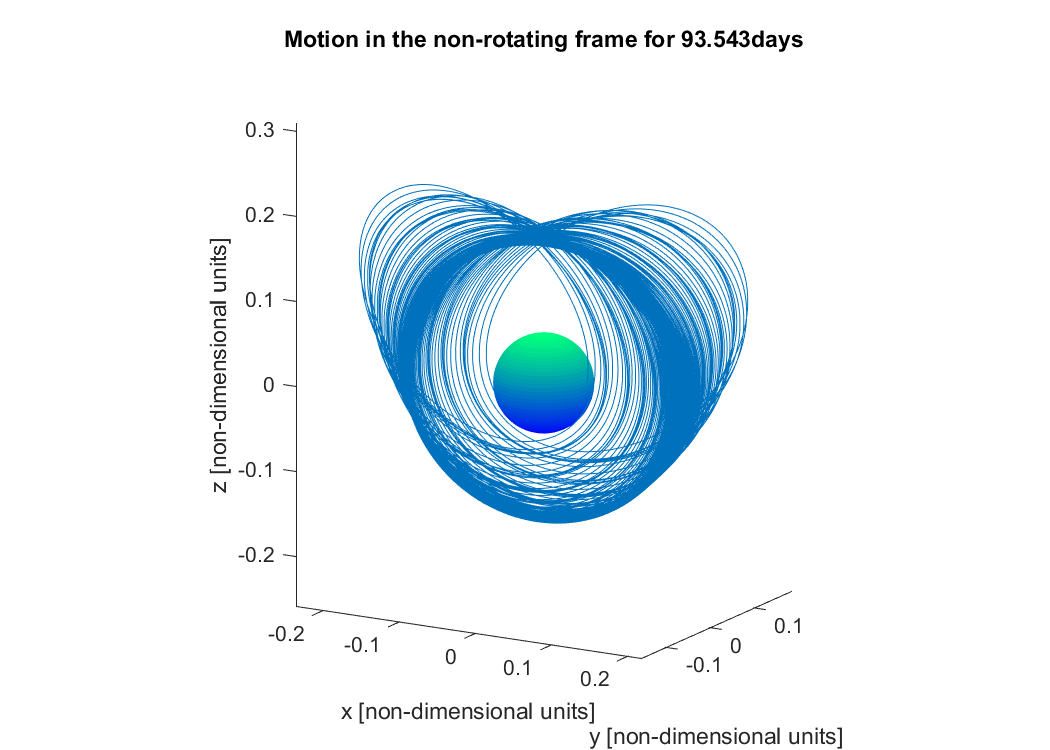
\includegraphics[height=3in]
	{figures/GanymedeESA/motionFixedFrame.png}
	\caption{Altitude profile for the mission compared with the prediction from the small eccentricity theory.}
	\label{fig:JUICEorbit}
\end{figure}

